\chapter{Sketch It, Make It: Overview}

The primary contribution of this thesis is the set of interaction
techniques implemented in a single design tool called Sketch It, Make
It (SIMI). SIMI is a modeling environment for laser cutter design that
recognizes short sequences of drawn input made with a stylus. Using
only freehand input, SIMI enables a designer to iteratively and
incrementally create precise laser cut models.

I am inspired by the potential of freehand drawing as the basis for
precision modeling for several reasons. Sketching is quick and can be
easily learned. It is simple and modeless: unlike structured editing
software, a designer need not set a pencil's mode to line, circle, or
anything else. I will show that given an appropriate set of
interaction methods, sketched input can provide enough information to
make a precise digital model.

There are several principles that guided SIMI's design and development.

\begin{itemize}
\item \textbf{Democratized design}: Freehand drawing is a skill that
  most people already have. It follows that a tool based on sketch
  based interaction should be usable by a majority of people. For this
  reason I target avocational designers, not professionals. 
\item \textbf{Sketch based}: The user should never feel obliged to set
  down their pen. In the past, many sketch based design tools have
  relied on keyboard input, or used interface widgets that are
  appropriate for mice but are uncomfortable to use with a stylus
  (e.g. hierarchic menus).
\item \textbf{Coherence of interaction techniques is key}: The tool
  presents a set of sketch based interaction techniques that work well
  together. Researchers commonly make toy systems that demonstrate one
  or two novel interaction techniques in isolation (e.g. my own prior
  work on Flow Selection~\cite{johnson-flow-selection}). But a useful
  tool has many individual techniques. The current system implements
  many techniques together to give an example of a way to make them
  work harmoniously.
\item \textbf{Useful and usable}: Last, the system lets people make
  real things in a real domain (namely, laser cut objects). The
  current implementation of the tool is efficient and highly
  responsive. In informal demonstrations, more than one person has
  noted that the system seems more like a commercial product than a
  research system. This is intentional.
\end{itemize}

\section{Rapid Fabrication and Laser Cutting}

Laser cutters are among the more common and affordable fabrication
machines. One can think of a laser cutter as a fast, strong, and
precise automated razor that cuts flat material (paper, wood, plastic,
textiles, etc.). 

% Price information: 
% 2001: 12,900 (ULS 25 watt)
% 2006: 9,995 (ULS 25 watt)
% 2010: 8,500 (ULS 25 watt)
% 2011: 6,850 (ULS 25 watt)
%
%   http://www.rcgroups.com/forums/showthread.php?t=16912 claims that
%   a 25-watt model from Universal Laser systems cost $12,900. Several
%   comments in that thread are in line with that price estimate for
%   home-garage-lab use.
%   http://www.microgeo-usa.com/ProductDetails.asp?ProductCode=universal-laser-VLS2.30
%   currently prices the ULS 25 watt 16x12 unit as costing $6,850.

% http://55-website.com/xo1/ulsinc/english/PDFs/EJ_VL_Article_Reprint.pdf is a press article from 2006 that prices the 25 watt laser at 10,000
\begin{figure}[b] %  figure placement: here, top, bottom, or page
   \centering
   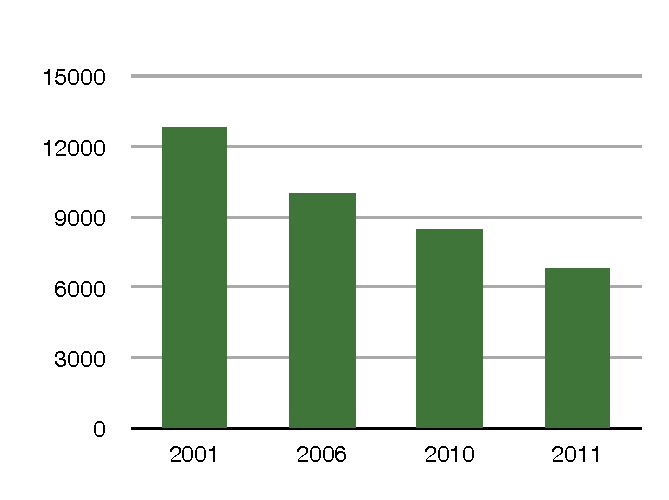
\includegraphics[width=3in]{img/prices.pdf} 
   \caption[Declining laser cutter prices]{Declining prices of Universal Laser Systems 25-Watt 16x12
     inch laser cutter (US Dollars).}
   \label{fig:prices}
\end{figure}


The price of laser cutters is quickly declining, making it possible
that more people have access to them. Figure~\ref{fig:prices} shows
prices for a comparable~25-Watt,~16''x12'' laser cutter model from
Universal Laser Systems (these values were found on hobbyist web
forums). While these data may not be exact, they do show the price of
desktop laser cutting machines has been cut by almost half in the past
ten years. While still out of reach for most people to afford, they
are becoming inexpensive enough for schools and hacker spaces to own.

Laser cut designs are composed of parts cut from solid, flat material
and assembled in various ways: laminated, notched, bolted together,
\textit{etc}. Various materials require different laser speed and
intensity settings to achieve a quality cut. The designe uses a
software application to specify part shapes for laser cutting. The
software outputs vector graphics called a ``cut file'' that defines
these shapes. As most joints have small margins of error, lengths,
angles, and relative position must be specified precisely so that
parts fit together properly.

Tools for designing laser cut objects must allow users to precisely
specify dimensions. Like a physical saw, the laser leaves a gap in its
wake, called a \textit{kerf}, (between 0.2mm and 0.5mm on a 40 watt
cutter). This is an important consideration when designing facets
whose tolerances are small with respect to kerf. A notch joint, for
example, is ineffective if it is 0.1 mm too large or small.


\section{Motivating Scenario: Pictureframe Holder}

\begin{figure}[h]
\centering 
\subfloat[] {
  \label{fig:example-1} 
  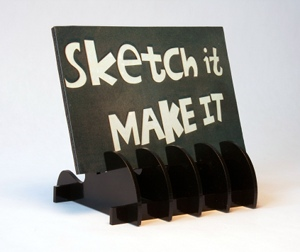
\includegraphics[width=0.45\linewidth]{img/simi-stand-withpic.jpg} 
}
\subfloat[] {
    \label{fig:example-2}
    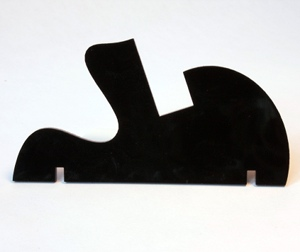
\includegraphics[width=0.45\linewidth]{img/simi-stand-part.jpg}
}
\caption{A picture stand \subref{fig:example-1} drawn and fabricated
  using SIMI. A single copy of the primary part is shown in
  \subref{fig:example-2}. }
\label{fig:simi-example}
\end{figure}

To introduce Sketch It, Make It we show how we use it to make the
picture stand shown in Figure~\ref{fig:simi-example}. We begin with
the idea of a stand with two horizontal rails as a base and a
five-part vertical support structure, joined with notches.

We first draw the rough profile of the vertical support piece using
curved and straight segments. SIMI captures our drawing, straightening
lines, smoothing curves, and connecting curved and straight segments.
 
After sketching the rough outlines of our two parts, we begin to
refine the design and make it precise.  We square the corners by
drawing right-angle braces (Figure~\ref{fig:motivating}a).  Now as we
adjust the shapes of the two parts by selecting and dragging endpoints
and re-shaping curves, SIMI maintains the right-angle constraints
we've established.
 
Next, we add notches to the two parts for the joints. We draw five
small notches on the base rail. For each notch we draw three lines
inside the outline of the part, and then use the erase gesture to
remove the residual outline segment (Figure~\ref{fig:motivating}b).
Then we indicate that both sides of the notch are to be the same
length: We draw tick marks on each segment, and right-angle braces to
keep the notch perpendicular to the edge of the part. The notches must
have exactly the right dimensions: too wide, the top parts will
wobble; too narrow and they will not fit. We size the notch by
overtracing its segments and entering fixed dimensions
(Figure~\ref{fig:motivating}c).
 
We drag the base part (twice) and the support part (five times) to
SIMI’s cut file area to prepare a PDF file for cutting, and then send
it to the laser cutter.  Finally we assemble the cut parts to make the
picture stand in Figure~\ref{fig:simi-example}.

\begin{figure}[h]
  \centering
  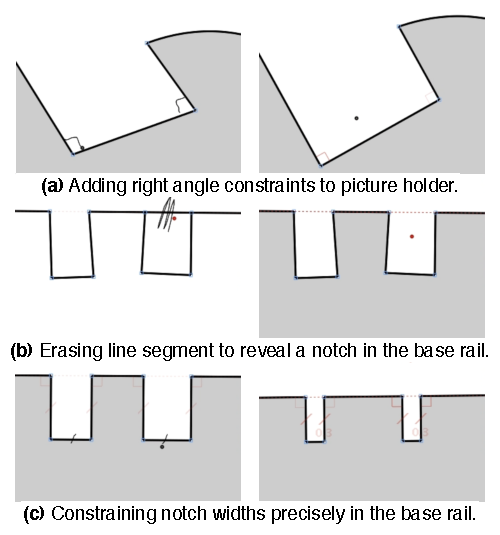
\includegraphics{img/motivating-example.pdf}
  \caption{Key steps taken when making the picture stand.}
  \label{fig:motivating}
\end{figure}


%% The second example is cribbed from the video. It is of the user
%% designing a picture frame holder. It involves:

%% \begin{itemize}
%% \item Using a tablet, most likely a `blind' tablet with separate
%%   display. Introduces hand/eye coordination issues.
%% \item Having the idea in the first place
%% \item Drawing roughly
%% \item Mistakes: errors (the user or the system makes errors) vs. ``on
%%   second thought'' mistakes
%% \item Adding details
%% \item Imagining 3D construction. Admit the tool should support this
%%   directly
%% \item Fabrication: making the cutfile, laser cutting, and assembling
%% \item (maybe) another iteration
%% \end{itemize}

\section{Technical Challenges Met By SIMI}

%% The above section describes the user's needs, and how the user
%% interacts with the system. This section introduces broadly how the
%% system is built to support those needs and interaction. Briefly, the
%% technical aspects are:

%% \begin{itemize}
%% \item Ink parsing (finding corners and segments, removing hooks)
%% \item Recognition (dynamic or post-hoc)
%%   \begin{itemize}
%%   \item Glyphs (akin to character recognition, like right angles)
%%   \item Gesture (recognizes grammatical patterns like erase or
%%     encircle)
%%   \end{itemize}
%% \item Disambiguation of recognized things
%% \item Data model and constraints
%%   \begin{itemize}
%%   \item User sketches things, system reates/maintains constraints
%%   \item Uses iterative, numerical relaxation method
%%   \item Only has X basic constraint types underlying everything
%%   \item High-level ``user constraints'' composed of low-level constraints
%%   \end{itemize}
%% \item Cutfile generation
%%   \begin{itemize}
%%   \item Basic typewriter algorithm. nothing fancy
%%   \item Scales things appropriately
%%   \item PDF output for Illustrator, SVG output for Ponoko (explain why
%%     format matters)
%%   \end{itemize}
%% \end{itemize}

%% From the user's perspective, SIMI gives a new kind of experience
%% because it:

%% \begin{itemize}
%% \item Is ``modeless''. Should describe the mode problem, why
%%   overcoming it is such an important thing, and why it is especially
%%   pertinent to sketch-based interaction. (because if we have modes, we
%%   are essentially on slippery-slope to MouseCAD)
%% \item Is incremental, rather than one-big-batch style recognition that
%%   is so popular
%% \item Uses ``more natural'' input. The pen is easier to manipulate
%%   than the mouse. Naturalness is a common term but is ultimately
%%   meaningless because all design tools are artificial. Could say it
%%   has less cognitive and ergonomic demands than modal, mouse-based
%%   tools
%% \item From a domain perspective it is not over featured, so it is
%%   clear how to proceed.
%% \end{itemize}
